\documentclass[a4paper,14pt]{extreport}
\usepackage[utf8]{inputenc}
\usepackage[T1]{fontenc}
%\usepackage{lmodern}
\usepackage[english, russian]{babel}
\usepackage{indentfirst}
\usepackage{amssymb,amsfonts,amsmath,mathtext,cite,enumerate,float}
\usepackage[dvips]{graphicx}
\usepackage{titlesec}

\usepackage{geometry}
\geometry{left=2cm}
\geometry{right=2cm}
\geometry{top=2cm}
\geometry{bottom=2cm}

\titleformat{\chapter}[block]{\normalfont\bfseries}{\thechapter}{20pt}{}{}
%\addto\captionsrussian{\renewcommand{\chaptername}{}}
%\renewcommand{\thechapter}{}

\graphicspath{{images/}}

% Title Page
\title{Введение в дипломную работу}
\author{Елисеев Владислав}

\makeatletter
\bibliographystyle{unsrt}
\renewcommand{\@biblabel}[1]{#1.} 
\makeatother
\parindent=1.5cm

\sloppy
\hyphenation{STan-ford}

\newenvironment{compactlist}{
    \begin{list}
    {{$\bullet$}}
    {
        \setlength\partopsep{0pt}
        \setlength\parskip{0pt}
        \setlength\parsep{0pt}
        \setlength\topsep{0pt}
        \setlength\itemsep{0pt}                        
    }
}{
    \end{list}
}

\begin{document}
\begin{titlepage}

\begin{center}
{\small
МОСКОВСКИЙ ГОСУДАРСТВЕННЫЙ УНИВЕРСИТЕТ имени М.В.~ЛОМОНОСОВА \\
ФАКУЛЬТЕТ ВЫЧИСЛИТЕЛЬНОЙ МАТЕМАТИКИ И КИБЕРНЕТИКИ \\
КАФЕДРА СИСТЕМНОГО ПРОГРАММИРОВАНИЯ
}
\end{center}

\vfill
\vfill
\begin{center}
\Large{\textbf{Введение в дипломную работу}} \\
~\\
\Large{Генерация моделей на унифицированном языке моделирования по описаниям предметных областей и задач планирования}
\end{center}
\vfill
\vfill
\vfill
\vfill
\begin{flushright}
Исполнитель: \\
студент 527 группы Елисеев Владислав
\end{flushright}
\vfill
\begin{flushright}
Научный руководитель: \\
к.ф.-м.н. Малышко Виктор Васильевич
\end{flushright}
  
\vfill
\vfill
\vfill
\vfill
\begin{center}
  Москва\\
  2013
\end{center}  
\end{titlepage}

\setcounter{page}{1}
\linespread{1.25}
\normalsize

	Одна из задач в области искусственного интеллекта - задача планирования. Планированием называется процесс выработки последовательности действий, позволяющей достичь цели \cite{norwig-ai}. Задача планирования часто встает у агентов, которым нужно найти последовательность действий, выполнив которые он достигнет некоторой своей цели. Агентом можно назвать все, что воспринимает свою среду с помощью некоторых датчиков и воздействует на нее с помощью некоторых механизмов. Примерами использования планирования может служить следующее: планирование управлением механическими приводами робота-мусоросборника, планирование распределения транспортных средств для перевозок различных видов топлива и сырья на нефтеперерабатывающем заводе. 


	Контекст задачи планирования, модель мира, в котором возникает задача, -- называется предметной областью. Они могут сильно отличаться друг от друга. Они могут быть детерминированными или стохастическими, статическими или динамическими, полностью наблюдаемыми или частично наблюдаемыми, и т.д. Многообразие моделей влияет на многообразие и сложность соответствующих алгоритмов решения задач планирования, на сложность и архитектуру агентов, на решение задачи планирования и её представление. 
	
	
	В работе рассматриваются полностью наблюдаемые, детерминированные, конечные, статические и дискретные модели мира, называемые иначе классическими моделями, или средами \cite{norwig-ai}. Для агентов, действующих в классических средах, характерно выделение трех основных понятий: \textit{состояние среды} (мира), \textit{действие} (механизмы воздействия на среду), \textit{цель} (целевое состояние мира), и встает необходимость определить, как представляется информация об этих понятиях. 
	
	В 1971 году был разработан формальный текстовый язык STRIPS \cite{strips} -- STanford Research Institute Problem Solver -- для представления задач планирования в классических средах, что послужило толчком к развитию классических алгоритмов планирования и планировщиков. В этом языке состояния задаются в виде некоторого набора фактов об объектах и отношениях между ними, которые считаются истинными в этом состоянии. Действия задаются с использованием набора ограничений на состояние (предусловие), и набора положительных и отрицательных фактов (эффекты). \textit{Предусловие} должно выполняться для того, чтобы применение действия было допустимым в данном состоянии. \textit{Эффект} задает то, как меняется состояние при применении действия -- положительные факты добавляются к состоянию, отрицательные -- удаляются. \textit{Цель}, или целевое состояние, задается как набор ограничений, которые должны быть удовлетворены в данном состоянии. Также в STRIPS вводится гипотеза замкнутости мира (CWA, \textit{Closed World Assumption}), которая означает, что факты, не перечисленные в описании состояния, считаются ложными.
	
	В 1987 году был предложен язык ADL -- Action Description Language \textit{(язык описания действий)} -- похожий на STRIPS, но включающий в себя несколько особенностей, из которых можно отметить следующие:
	\begin{itemize}
	    \item предположение об открытом мире - факты, не перечисленные в состоянии, считаются неизвестными;
	    \item возможность использования кванторов и дизъюнктов для задания цели;
	    \item возможность использования условных эффектов;
	    \item наличие встроенного предиката равенства для сравнения объектов;
	    \item типизация переменных;
	    \item и т.д.
	\end{itemize}
    
    Помимо	языков STRIPS и ADL, вдохновленные ими, развивались и другие текстовые языки представления знаний, каждый из которых использовал свой синтаксис, семантику и другие возможности. В 1988 году появился язык PDDL\cite{pddl3} -- Planning Domain Definition Language \textit{(язык описания предметных областей и задач планирования)} -- как попытка стандартизации существующих на тот момент языков описания предметных областей и задач планирования. Также это сделало возможным создание IPC -- International Planing Competition -- международных соревнований по созданию планировщиков.  
    
    Рассмотрим примеры PDDL-описаний для игры <<Sokoban>> \textit{(пер. кладовщик)}, предложенные на IPC в 2008 году. Мир в данной игре представляет собой некоторую область, поделенную на клетки одинакового размера, которые бывают проходимыми и непроходимыми (фактически, это лабиринт). В некоторых клетках расположены предметы -- это могут быть камни, сундуки, ключи и т.п. Другие клетки имеют пометки ""целевые"" -- углубления в полу для камней, замочные скважины для ключей (для люков в полу) и т.п. Количество целевых клеток и предметов совпадает. В игре есть игрок, который передвигается по клеткам лабиринта. В одной клетке не могут находиться игрок и предмет одновременно. Целью игрока является расположить все предметы по их целевым клеткам, причем не важно, в каком порядке и каким образом они будут расположены в целевых клетках. За один ход игрок может передвинуть предмет, находящийся в соседней клетке по направлению движения, в клетку за ней, если она свободна и проходима. Фрагмент описания предметной области игры <<Sokoban>> представлен далее: 

\linespread{0.80}    
\begin{verbatim}
(define (domain sokoban-sequential)
  ;; определяем предметную область
  
  (:requirements :typing :action-costs)
  ;; указываем какие возможности PDDL используются
  ;; :typing -- используется типизация переменных
  ;; :action-costs -- действия имеют стоимость
  
  (:types thing location direction - object
          player stone - thing)
  ;; описываем иерархию типов: thing, location, direction --
  ;; наследуют базовый тип object
  ;; player, stone -- наследуют уже определенный тип thing
  
  ;; далее описываются предикаты
  (:predicates (clear ?l - location)
      ;; -- свободна ли локация
      (at ?t - thing ?l - location) 
      ;; -- находится ли предмет в локации
      (at-goal ?s - stone)          
      ;; -- находится ли камень в целевой локации
      (IS-GOAL ?l - location)       
      ;; -- является ли локация целевой и т.д.
      (IS-NONGOAL ?l - location)
      (MOVE-DIR ?from ?to - location ?dir - direction))
             
  
  (:functions (total-cost) - number)
      ;; total-cost -- функция без аргументов, 
      ;; возвращает одно число -- суммарную стоимость
      ;; примененных функций

  ;; далее следуют описания действий
  (:action move
      ;; действие -- двигаться
   :parameters (?p - player ?from ?to - location ?dir - direction)
      ;; четыре параметра, ограничение на типы
          
   :precondition (and (at ?p ?from)
                      (clear ?to)
                      (MOVE-DIR ?from ?to ?dir)
                      )
      ;; предусловия -- игрок находится в локации ?from,
      ;; локация ?to свободна, а направление перемещения
      ;; из локации ?from  в ?to совпадает с ?dir
   :effect       (and (not (at ?p ?from))
                      (not (clear ?to))
                      (at ?p ?to)
                      (clear ?from)
                      )
       ;; эффект от применения действия --
       ;; ?p не находится в локации ?form,
       ;; ?to больше не свободна,
       ;; ?p находится в локации ?to,
       ;; локация ?from теперь свободна
   )
   
   (:action push-to-nongoal
       ;; действие -- продвинуть камень в не целевую локацию
   :parameters (?p - player ?s - stone
                ?ppos ?from ?to - location
                ?dir - direction)
   :precondition (and (at ?p ?ppos)
                      (at ?s ?from)
                      (clear ?to)
                      (MOVE-DIR ?ppos ?from ?dir)
                      (MOVE-DIR ?from ?to ?dir)
                      (IS-NONGOAL ?to)
                      )
   :effect       (and (not (at ?p ?ppos))
                      (not (at ?s ?from))
                      (not (clear ?to))
                      (at ?p ?from)
                      (at ?s ?to)
                      (clear ?ppos)
                      (not (at-goal ?s))
                      (increase (total-cost) 1)
                      )
   )
   <...>
  )
\end{verbatim}
\linespread{1.25}

    Описание задачи на языке PDDL для данной предметной области представлено ниже с вырезанными фрагментами, так как оно требует описания \textbf{всех} объектов, их отношений между собой \textbf{со всеми} деталями и т.д., что может занять довольно много места:
  
\newpage
\linespread{0.80}
\begin{verbatim}
;;   #######
;; # #     #
;; # # # # #
;;   # @ $ #
;; ### ### #
;; #   ### #
;; # $  ##.#
;; ## $  #.#
;;  ## $  .#
;; # ## $#.#
;; ## ## #.#
;; ### #   #
;; ### #####

(define (problem p109-microban-sequential)
  ;; определяем задачу
  
  (:domain sokoban-sequential)
      ;; указываем предметную область, для которой
      ;; сформулирована задача  
  
  (:objects
    ;; перечисляем все объекты,
    ;; кторые фигурируют в задаче
    
    dir-down - direction
    dir-left - direction
    dir-right - direction
    dir-up - direction
    player-01 - player
    pos-01-01 - location
    pos-01-02 - location
    pos-01-03 - location
    pos-01-04 - location    
    <..>
  (:init
    ;; формулируем начальное состояние системы  
    ;; задаем значение предикатов на объектах системы
    (at player-01 pos-05-04)
    (at stone-01 pos-07-04)
    (at stone-02 pos-03-07)
    <..>
    (IS-GOAL pos-08-07)
    (IS-GOAL pos-08-08)
    (IS-GOAL pos-08-09)
    (IS-GOAL pos-08-10)
    (IS-GOAL pos-08-11)
    (IS-NONGOAL pos-01-01)
    (IS-NONGOAL pos-01-02)
    (IS-NONGOAL pos-01-03)
    (IS-NONGOAL pos-01-04)
    <..>
    (MOVE-DIR pos-01-01 pos-02-01 dir-right)
    (MOVE-DIR pos-01-04 pos-02-04 dir-right)
    (MOVE-DIR pos-02-01 pos-01-01 dir-left)
    <..>
    (clear pos-01-01)
    (clear pos-01-04)
    (clear pos-01-09)
    (clear pos-02-01)
    <..>
  )
  
  ;; теперь  формулируем ограничения на целевое состояние
  ;; все камни должны располагаться в целевых локациях
  (:goal (and
    (at-goal stone-01)
    (at-goal stone-02)
    (at-goal stone-03)
    (at-goal stone-04)
    (at-goal stone-05)
  ))
  
  ;; формулируем метрику, с помощью которой
  ;; оценивается качество планов
  (:metric minimize (total-cost))
)    
    
\end{verbatim}
\linespread{1.25}

    PDDL имеет широкие возможности для описания знаний о моделях мира и задачах планирования. Он развивается и по сей день, в последнее время двигаясь в направлении представления знаний, близкому к объектному.

    Объектное представление -- представление, которое позволяет оперировать понятиями объекта, связанных с ним данных и методов, как с единым целым. Сейчас наряду с текстовыми языками представления знаний используются и графические языки, например UML\cite{rambo-uml2} -- Unified Modeling Language \textit{(унифицированный язык моделирования)}. Данный язык хорошо подходит для записи знаний в объектном представлении. 
    
    Язык UML был создан для удовлетворения нужд программной индустрии, но его возможности оказались шире, поэтому он используется и в других областях. Например, его можно использовать для представления знаний систем планирования в виде UML моделей. Для создания UML моделей существует множество редакторов, что делает возможность задания знаний среды и задачи планирования в объектном представлении более привлекательной.
    
    В данной дипломной работе рассматривается следующая задача: по текстовым описаниям на языке PDDL требуется сгенерировать соответствующие им UML модели. Получение UML-представления может быть полезно, так как:
    \begin{itemize}
        \item UML модели более наглядны, составлять UML базы знаний могут эксперты, не знакомые с PDDL и его устройством;
        \item UML модель может быть отредактирована в графическом редакторе, затем оттранслирована в PDDL\cite{mal-manz};
        \item можно использовать инструменты UML-валидации и исполнения для проверки корректности знаний\cite{use, gladkova}; 
        \item по UML-описанию предметной области могут быть сформулированы задачи для этой предметной области\cite{dolotkazin}.
    \end{itemize}


    Таким образом, предполагается создать программное средство, которое будет автоматизировать преобразование PDDL-описаний предметных областей и задач планирования в  UML-модели. На вход средство будет получать PDDL-описания. Знания в этом представлении состоят из описания предметной области (типов, предикатов, функций, операций, а также их предусловий и эффектов), и описаний задач, каждая из которых представлена в виде описаний начальных и конечных состояний, требований предъявляемых к решению задачи. 
Создаваемое средство должно преобразовывать данное представление знаний, и на его выходе должно получиться объектное представление тех же знаний. В ходе работы средства к представлению будет применяться ряд преобразований. Пусть $T$ -- описываемое преобразование, $T: A \to B$, $A$ -- база знаний в исходном (текстовом PDDL-представлении), $B$ -- база знаний в целевом представлении (в виде UML-модели). Преобразование должно обладать следующими свойствами:
    \begin{enumerate}
        \item Любой PDDL-тип $C \in A \rightarrow C' \in B$, где $C'$ -- UML-класс (Рис.~\ref{img:property-types});

\begin{figure}[H]
    \hfill
    \begin{minipage}[h]{0.40\linewidth}
        {\raggedright
        \begin{verbatim}
    (:types
        thing - object
    )
        \end{verbatim} 
        }
    \end{minipage}
    \hfill
    $\rightarrow$
    \hfill
    \begin{minipage}[h]{0.45\linewidth}
        \center{
\includegraphics[width=0.5\linewidth]{Class_1.eps}}
    \end{minipage}
    \caption{Пример преобразования типов}
    \label{img:property-types}
\end{figure}

        \item Отношения между PDDL-типами $C_1, C_2 \in A$ должны переводиться в отношения между UML-классами $C_1', C_2' \in B$, с использованием атрибутов, ассоциаций и др. (Рис.~\ref{img:property-relations}); 
        
\begin{figure}[H]
    \hfill
    \begin{minipage}[h]{0.40\linewidth}
        {\raggedright
        \begin{verbatim}
    (:types
        thing - object
        stone - thing
    )
        \end{verbatim} 
        }
    \end{minipage}
    \hfill
    $\rightarrow$
    \hfill
    \begin{minipage}[h]{0.45\linewidth}
        \center{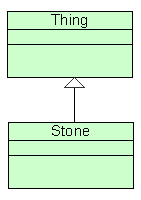
\includegraphics[width=0.5\linewidth]{Class_2}}
    \end{minipage}
    \caption{Пример преобразования отношений}
    \label{img:property-relations}
\end{figure}

        \item Любой PDDL-объект $o \in A \to o' \in B$, где $o'$ -- экземпляр UML-класса и если $C \in A$ -- некоторый класс, то $C \to C' \in B, \Rightarrow o' \in C'$;
        \item Любое PDDL-состояние $S \in A \to S' \in B$, где $S'$ -- состояние, описываемое UML. Причем:
        \begin{enumerate}
            \item  Для любого PDDL-объекта в этом состоянии $o \in S$, то в $S'$ должен существовать объект $o' \in B$, $o'$ - образ объекта $o$;
            \item  Если PDDL-объекты $o_1, o_2 \in A$ связаны конструкциями, то их образы $o'_1, o'_2 \in B$ должны быть связаны соответствующими конструкциями, если это возможно;
             
        \end{enumerate}
        \item Любое действие $a \in A$ имеет образ $a' \in B$, причем если в результате применения действия $a$ в состоянии $s_1 \in A$ получается $s_2 = apply(a, s_1), s_2 \in A$, то образы $s_1' \in B$ и $s_2' \in B$ связаны аналогичным соотношением $s_2' = apply(a', s_1')$ (Рис.~\ref{img:property-actions});
        
\begin{figure}[H]
    \begin{minipage}[h]{1\linewidth}
        {\raggedright
        \small
        \begin{verbatim}
   (:action move
   :parameters (?p - player ?from ?to - location ?dir - direction)        
   :precondition (and (at ?p ?from)
                      (clear ?to)
                      (MOVE-DIR ?from ?to ?dir)
                      )
   :effect       (and (not (at ?p ?from))
                      (not (clear ?to))
                      (at ?p ?to)
                      (clear ?from)
                      )
   )
        \end{verbatim} 
        }
    \end{minipage} \\
    \vfill
    {\centering $\downarrow$ \\ }  
    \vfill
    \begin{minipage}[h]{1\linewidth}
        \center{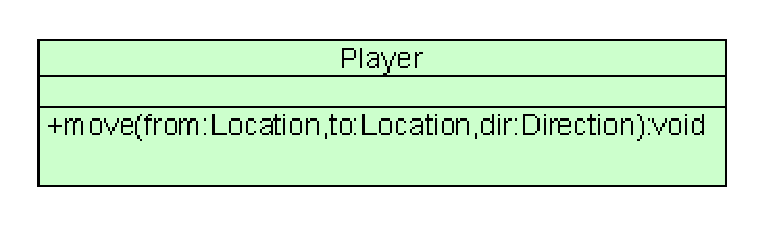
\includegraphics[width=0.8\linewidth]{Class_3}}    
    \end{minipage} \\
    \vfill
    {\centering $+$ \\ \medskip } 
    
        {\centering OCL\cite{ocl} ограничения на метод \\ \bigskip} 
        
        \hfill
        \begin{minipage}[h]{0.43\linewidth}
           {\centering <<pre>> \\}  
           {\raggedright
            \small
        
            \begin{verbatim}
this.at == from and 
to.isClear and
LocDirRelation->
exists(LocDirRelation{from, to, dir})
    
            \end{verbatim}
           }      
           
        \end{minipage}    
        \hfill            
        \begin{minipage}[h]{0.43\linewidth}
           {\centering <<effect>> \\}  
           {\raggedright
            \small
        
            \begin{verbatim}
    ! this.at == from and
    ! to.isClear and
    this.at == to and 
    from.isClear
            \end{verbatim}
           }     
           \vfill 
        \end{minipage}

    \caption{Пример преобразования действий}
    \label{img:property-actions}
\end{figure}      

    \item PDDL-представление любой задачи (начальное состояние и цель) должно переводиться в соответствующее UML-представление c сохранением свойств объектов и отношений между ними, как описано в предыдущих пунктах.
    \end{enumerate}
    
    Одной из сред поддержки процессов, связанных с планированием, является среда itSIMPLE\cite{itsimple}. В данной среде была решена обратная задача: трансляция UML моделей в PDDL описания. Для этого было предложено использовать специальную семантику некоторых UML-элементов. Так или иначе, средство не решает задачу, поставленную в данной работе.
    
    Подавляющее большинство инструментов, реализующих преобразование каких-либо текстовых данных в UML-модели, существует для работы с языками программирования, как правило, объектно-ориентированными, а не с языками представления знаний. Поэтому, использование этих инструментов для решения поставленной задачи невозможно. 
    
    Среди инструментов, работающих не только с языками программирования, можно выделить MoDosco. Данный инструмент позволяет создавать модели различных систем, используя специальные Discoverer'ы, которые на данный момент существуют в основном для Java-кода и JAR-архивов. Кроме того, данный проект находится в инкубаторе и о создании PDDL-Discoverer'ов говорить не приходится. 
    

    

\newpage
\begin{thebibliography}{00}

\bibitem{norwig-ai}
\textbf{Рассел С., Норвиг П.} \textit{Искусственный интеллект: современный подход, 2-е изд.} М. : Вильямс, 2006. 1408 с.

\bibitem{strips}
\textbf{Fikes R., Nilsson N.} \textit{STRIPS: a new approach to the application of theorem
proving to problem solving // Artificial Intelligence}. 1971. 2. P. 189-208.

\bibitem{pddl3}
\textbf{Gerevini, A., Long, D.} \textit{Plan constraints and preferences in PDDL3.} Technical Report, Univ. Brescia, Italy, 2005. 12p.

\bibitem{rambo-uml2}
\textbf{Рамбо Дж., Блаха М.} \textit{UML 2.0. Объектно-ориентированное моделирование и разработка, 2-е изд.} СПб. : Питер, 2007

\bibitem{mal-manz}
\textbf{Малышко В. В., Манжосов А. В.} \textit{Решение задач инженерии знаний средствами объектно-ориентированной инженерии программного обеспечения // Программные системы и  инструменты. Тематический сборник No 13.} М. : Изд-во факультета ВМиК МГУ, 2012. стр. 44-54.

\bibitem{use}
\textbf{Gogolla M., Büttner F., Richters M.} \textit{USE: A UML-Based Specification Environment for Validating UML and OCL.} Science of Computer Programming, vol. 69, no. 1-3. 2007. pp. 27-34.

\bibitem{gladkova}
\textbf{Гладкова О. А.} \textit{Визуализация и валидация планов при помощи объектных моделей.} Дипломная работа. М. : МГУ ВМК, кафедра системного программирования, семинар <<Планирование целенаправленной деятельности>>, 2013.

\bibitem{dolotkazin}
\textbf{Долотказин Ю. В.} \textit{Генерация описаний задач планирования по объектной модели предметной области.} Дипломная работа. М. : МГУ ВМК, кафедра системного программирования, семинар <<Планирование целенаправленной деятельности>>, 2013.

\bibitem{ocl}
\textbf{Warmer, Kleppe.} \textit{The Object Constraint Language: Getting Your Models Ready for MDA, Second Edition.} Addison-Wesley, 2003.

\bibitem{itsimple}
\textbf{Vaquero T. S., Tonaco R. et al.} \textit{itSIMPLE4.0: Enhancing the Modeling
Experience of Planning Problems.} Proceedings of the ICAPS 2012 System
Demonstration, São Paulo : s.n., 2012. pp. 11-14.



\end{thebibliography}

\end{document}          
